\documentclass[border=2mm]{standalone}

\usepackage{tikz}
\usetikzlibrary{mindmap,trees,shadows,backgrounds}

\begin{document}

%\begin{figure}[h]
%\makebox[\textwidth][c]{
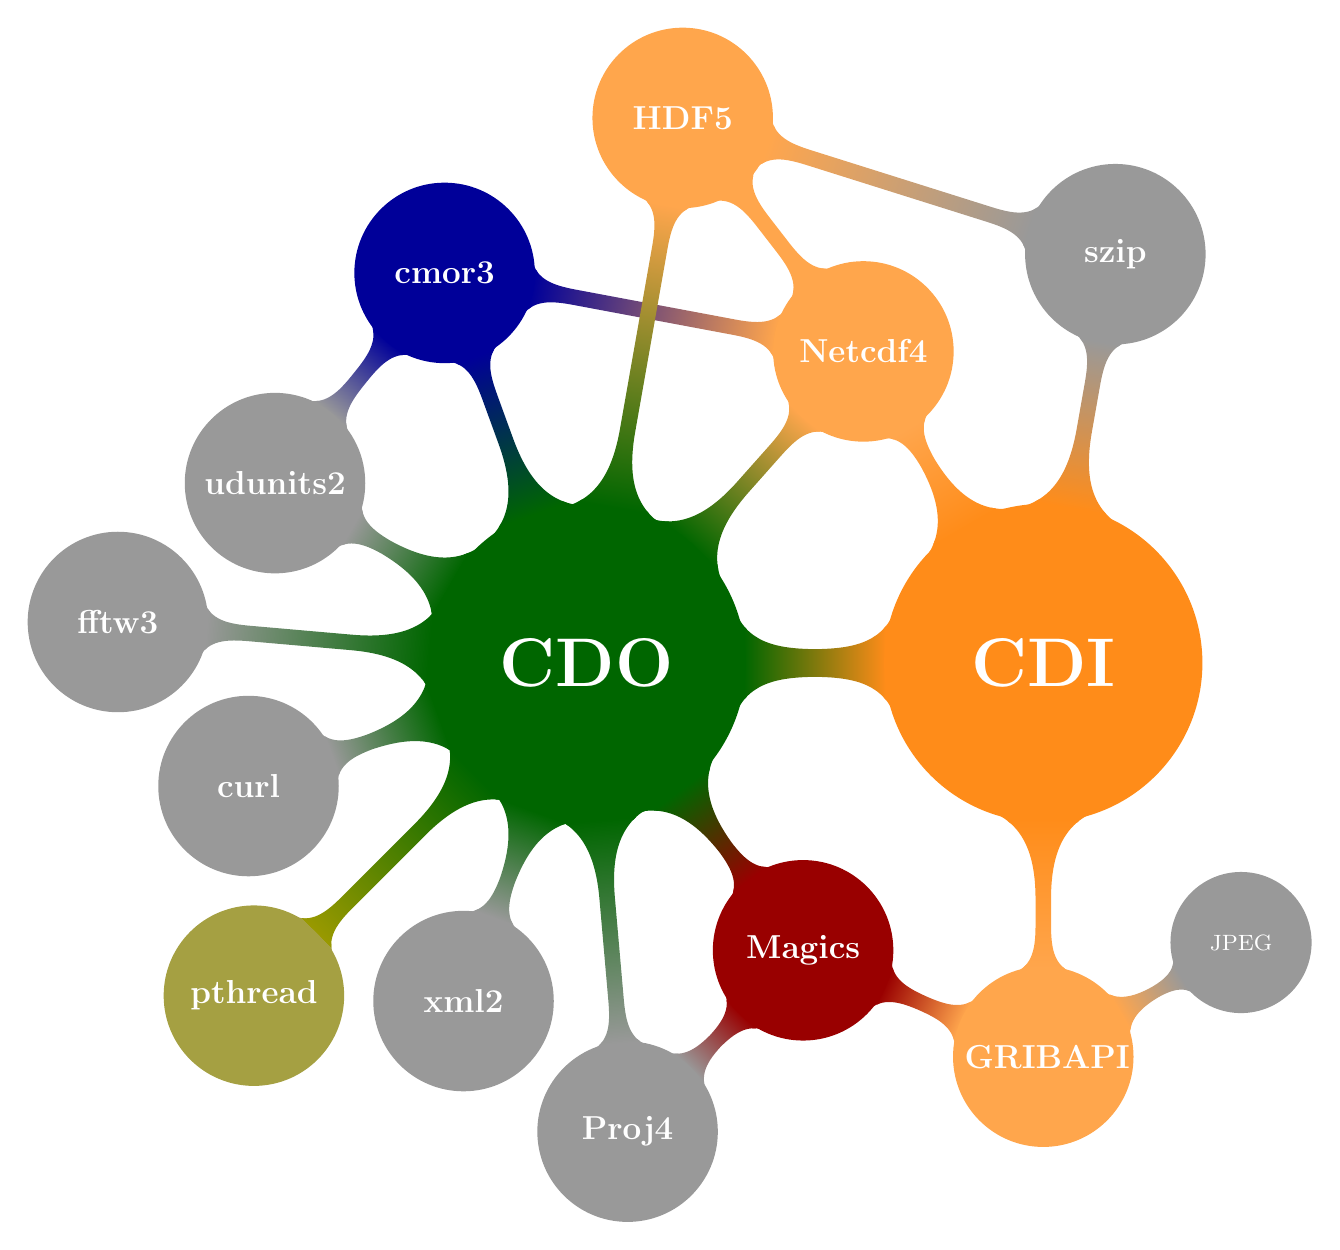
\begin{tikzpicture}
[ every annotation/.style = {draw, fill = white, font = \Large}]
%[decoration={start radius=1cm, end radius=.5cm,amplitude=3mm,angle=30}]

% Define experience colors
\colorlet{cdocolor}{green!40!black}
\colorlet{cdicolor}{orange!90}
\colorlet{netcolor}{orange!70}
\colorlet{hdfcolor}{orange!70}
\colorlet{gribcolor}{orange!70}
\colorlet{cmorcolor}{blue!60!black}
\colorlet{magiccolor}{red!60!black}
\colorlet{pthreadcolor}{yellow!60!black}
\colorlet{libcolor}{black!40}
%\colorlet{zipcolor}{blue!80!white!60!green}
\colorlet{zipcolor}{black!40}

  % \path[mindmap,concept color=black!40,text=white,
  %   every node/.style={concept,circular drop shadow},
  %   root/.style    = {concept color=black!40,
  %     font=\large\bfseries,text width=10em},
  %   level 1 concept/.append style={font=\Large\bfseries,
  %     sibling angle=50,text width=7.7em,
  %   level distance=15em,inner sep=0pt},
  %   level 2 concept/.append style={font=\bfseries,level distance=9em},
  % ]

%%%%%%%%%%% CDO
  \path[mindmap,concept color=cdocolor,text=white,font=\Huge\bfseries,
   % every node/.style={concept,circular drop shadow}
   % root/.style    = {concept color=black!40, font=\Huge\bfseries,text width=10em},
   level 1 concept/.append style={font=\large\bfseries,level distance=10em},
   ]

 % \node[concept] {Statsitiker\\ WG}
  %  child[concept color=cdocolor, grow=right]{ node[concept]{Janna}};

    node[concept](cdo) at (1,0){CDO}
            child [grow =  -53, concept color = magiccolor, level distance=130] { node[concept](magics){Magics}}
            child [grow =  -85, concept color = libcolor, level distance=170] { node[concept](proj) {Proj4}}
            child [grow = -110, concept color = libcolor, level distance=130] { node[concept](xml) {xml2}}
            child [grow = -135, concept color = pthreadcolor, level distance=170] { node[concept](pthread) {pthread}}
            child [grow = -160, concept color = libcolor, level distance=130] { node[concept](curl) {curl}}
            child [grow =   175, concept color = libcolor, level distance=170] { node[concept](fft) {fftw3}}
            child [grow =   150, concept color = libcolor, level distance=130] { node[concept](udunits){udunits2}}
            child [grow =   110, concept color = cmorcolor, level distance=150] { node[concept](cmor){cmor3}}
            child [grow =    80, concept color = hdfcolor, level distance=200] { node[concept](hdf){HDF5}}
       ;

%%%%%%%%%% CDI
  \path[mindmap,concept color=cdicolor,text=white,font=\Huge\bfseries,
    level 1 concept/.append style={font=\large\bfseries},
 %   level 2 concept/.append style={font=\large\bfseries},
  ]

    node[concept](cdi) at (6.8,0){CDI}
            child [grow =    120, concept color = netcolor, level distance=130] { node[concept](netcdf){Netcdf4}}
            child [grow =      80, concept color = zipcolor, level distance=150] { node[concept](szip){szip}}
            child [grow =   -90, concept color = gribcolor] { node[concept](gribapi){GRIBAPI}
               child [grow =    30, concept color = zipcolor] { node[concept](jpeg){JPEG} }
           }
      ;

%%%%%%%%%% MAKING SECONDARY CONNECTIONS 
   \newcommand{\concdotocdi}{to[circle connection bar switch color=from (cdocolor) to (cdicolor)]}
   \newcommand{\concdotonetcdf}{to[circle connection bar switch color=from (cdocolor) to (netcolor)]}
   \newcommand{\conhdftonetcdf}{to[circle connection bar switch color=from (hdfcolor) to (netcolor)]}
   \newcommand{\conhdftoszip}{to[circle connection bar switch color=from (hdfcolor) to (zipcolor)]}
   \newcommand{\concmortonetcdf}{to[circle connection bar switch color=from (cmorcolor) to (netcolor)]}
   \newcommand{\concmortoudunits}{to[circle connection bar switch color=from (cmorcolor) to (libcolor)]}
   \newcommand{\conmagicstogribapi}{to[circle connection bar switch color=from (magiccolor) to (gribcolor)]}
   \newcommand{\conmagicstoproj}{to[circle connection bar switch color=from (magiccolor) to (libcolor)]}
   \begin{pgfonlayer}{background} \path [style={sibling angle=80}] (cdo) \concdotocdi (cdi); \end{pgfonlayer}
   \begin{pgfonlayer}{background} \path (cdo) \concdotonetcdf (netcdf); \end{pgfonlayer}
   \begin{pgfonlayer}{background} \path (hdf) \conhdftonetcdf (netcdf); \end{pgfonlayer}
   \begin{pgfonlayer}{background} \path (hdf) \conhdftoszip (szip); \end{pgfonlayer}
   \begin{pgfonlayer}{background} \path (cmor) \concmortonetcdf (netcdf); \end{pgfonlayer}
   \begin{pgfonlayer}{background} \path (cmor) \concmortoudunits (udunits); \end{pgfonlayer}
   \begin{pgfonlayer}{background} \path (magics) \conmagicstogribapi (gribapi); \end{pgfonlayer}
   \begin{pgfonlayer}{background} \path (magics) \conmagicstoproj (proj); \end{pgfonlayer}

\end{tikzpicture}
%}
%\end{figure}

\end{document}
